\documentclass[12pt,a4paper]{article}
\usepackage[utf8x]{inputenc}
\usepackage[spanish] {babel}
%\usepackage{ucs}
\usepackage{makeidx}
\usepackage[pdftex]{graphicx}

\title { \textbf{Propuesta de Trabajo Profesional}}
\date{2do cuatrimestre de 2010}
\author{\textbf{Ciancio Alessio, Mauro Lucas} \\
		\textbf{Gilioli, Leandro Ezequiel}	  \\
		\texttt{\{maurociancio,legilioli\}@gmail.com}
	}

\begin{document}
\maketitle
\tableofcontents
\newpage

	\section{Integrantes}

A continuación se listan los alumnos que desarrollaron esta propuesta y se incluye sus datos personales:

	\begin{itemize}
		\item Ciancio Alessio, Mauro Lucas. \\
		      Padrón 86.357.
		\item Gilioli, Leandro Ezequiel. \\
		      Padrón 86.075.
	\end{itemize}

El profesor tutor de este trabajo profesional es Pablo Cosso.

	\section{Contexto}

	En el presente documento se definirá el plan de proyecto para la propuesta realizada en el documento de visión titulado ``Visión Trabajo Profesional" (para más información ver \cite{visiontpprof}). 

	Dentro del mismo se definirán entre otros los siguientes puntos: alcance, planificación, riesgos y criterios de calidad. 

	Este documento servirá de soporte en el proceso de desarrollo del producto y definirá criterios para medir el avance del proyecto de forma objetiva.	
		
	\section{Objetivo del proyecto}

El objetivo del proyecto es obtener un producto de software que permita a los usuarios elaborar documentos de texto de forma concurrente y en tiempo real. El producto se dividirá en dos sub productos de menor tamaño: el primero permitirá la edición colaborativa de texto usando un software independiente de cualquier otra aplicación. El segundo comprenderá la integración con un entorno de desarrollo integrado (IDE \cite{ide}).

El nombre producto será ``Parallel Editor".

A su vez, se pretende desarrollar el producto siguiendo los criterios de calidad que se definen más adelante en este documento.

También se desarrollará documentación de usuario y técnica del producto de modo que sea posible la extensión e incorporación a otras plataformas e IDE's.

El producto será desarrollado teniendo en cuenta la integración del mismo en otros contextos, por lo que se podrá observar una vez finalizado que los dos subproductos reutilizan un gran porcentaje del código fuente desarrollado una sola vez. Este punto es importante y es considerado en los requerimientos no funcionales.	
	
	\section{Necesidades del cliente / Mercado}
	
	Se necesita una herramienta con las siguientes características:
	\begin{itemize}
		\item La posibilidad de que dos o más personas editen un mismo documento en tiempo real sin la necesidad de estar fisicamente en el mismo lugar.
		\item Provisión al usuario de un mecanismo sencillo para la iniciación de una sesión de edición.
		\item Bajo costo de infraestructura al no requerir un servidor central dedicado para este producto.
		\item Resolución transparente de los posibles conflictos de la naturaleza concurrente de la edición en tiempo real.
		\item Independencia de una conexión a Internet para su disponibilidad. Esto se traduce a que el producto pueda funcionar en una red LAN que no esté conectada a internet.
	\end{itemize}

	\section{Competencia}

En esta sección se describirán productos existentes en el mercado y se compararán con la presente propuesta:

	\subsection{Google Docs y Google Wave}

	Provee la posibilidad de editar en tiempo real concurrentemente documentos con formato utilizando un navegador compatible. Posibilita la participación de múltiples usuarios en línea.

	Sin embargo, su mayor desventaja consiste en la dependencia de una conexión a internet para la disponibilidad del servicio, no es posible hasta ahora, la utilización del mismo en una red LAN privada.

	 Además es sólo utilizable a través de la interfaz web del navegador por lo cual su integración con herramientas de terceros no es posible. Cabe aclarar que Google ha abandonado el desarrollo de Google Wave.

	Las URL de éstos productos son las siguientes: http://wave.google.com y http://docs.google.com.

	\subsection{BeeWeeVee}

	Framework para la integración de funcionalidades de colaboración en tiempo real en aplicaciones. Se provee como un software development kit para el desarrollo sobre la plataforma .NET. Por este motivo, si bien abarca gran cantidad de desarrollos que hacen uso de dicha plataforma, no cubre totalmente el espacio de potenciales aplicaciones ya que las aplicaciones que no se desarrollan en .NET no pueden integralo.

	Es de licencia libre para uso académico y aplicaciones open source, aunque tiene un costo para la integración en desarrollos privados.

	La URL de este producto es: http://www.beweevee.com.

	\subsection{COLA - Eclipse Plugin}

	COLA es un plugin para la integración con Eclipse que permite la colaboración en tiempo real de los usuarios para editar un mismo documento de código fuente. Está desarrollado en Java y está basado en el proyecto Eclipse Communication Framework (ECF). Su principal desventaja es la dependencia con el mismo y por otra parte, limita la cantidad de usuarios que pueden participan en una sesión de edición de código a dos participantes.

	\subsection{Comparación con la presente propuesta}
El producto a desarrollar estará orientado a cubrir aquellos aspectos que las soluciones antes descriptas dejan de lado. Se pretenden liberar el código fuente bajo una licencia open-source, garantizar la portabilidad del mismo usando tecnologías que corren sobre la máquina virtual de Java, lograr independencia sobre otros frameworks o componentes de software y lograr que pueda haber mas de dos participantes en la misma sesión de edición.

Estas características descriptas determinarán los requerimientos funcionales y no funcionales que se describirán mas adelante.

	\section{Alcance}
   En la visión del proyecto se listaron las posibles funcionalidades que podría incluir el producto, de ellas se seleccionarán las siguientes para ser completadas en el presente proyecto:
   
	\subsection{Núcleo}
	Consiste en una biblioteca de software que proveerá servicios de apertura y cierre de sesiones de desarrollo. Se encargará de la administración de los participantes de la sesión de desarrollo, recibiendo e informando los cambios indroducidos por cada uno de ellos y resolviendo los conflictos que se produzcan debido a la concurrencia.
	
	También el núcleo ofrecerá una API de modo que las aplicaciones que requieran un servidor embebido puedan usar la misma.

	\subsection{API Cliente}
	Comprenderá la biblioteca que se encarga de implementar el protocolo de comunicación de un participante de la sesión con el núcleo del sistema. Esta API sera utilizada tanto por el cliente GUI como también por el plugin.

	\subsection{Interfaz gráfica}
	Se desarrollará una pequeña aplicación independiente que permitirá la edición colaborativa utilizando las APIs antes mencionadas.

	\subsection{Integración con IDE}
	Se desarrollará un agregado o plug-in para integrar la funcionalidad de desarrollo colaborativo en tiempo real dentro del IDE Eclipse.

	\section{Estimación}

	Se realiza una estimación de esfuerzo para el producto con el objetivo de fijar una fecha de liberación. La herramienta que se utilizó fue WBS \cite{wbs}.

	En cada tarea detallada en la WBS se tuvo en cuenta el esfuerzo necesario de análisis, desarrollo, documentación y testing.

	En la figura \ref{WBS} se puede observar la WBS para el producto. Se observan las columnas que muestran el nombre de la tarea y la estimación de esfuerzo para la misma.

	\begin{figure}[!ht]
		\begin{center}
			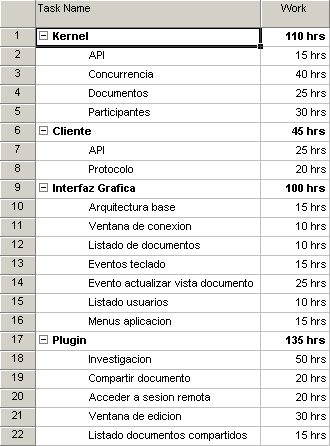
\includegraphics[width=9cm]{wbs.png}
			\caption{\label{WBS} Estimación de esfuerzo }
		\end{center}
	\end{figure}

	El valor final de la estimación es 390 horas hombres (HH). Las horas hombre son horas hombres productivas.

	\section{Planificación}

	Se cuenta con dos recursos con una disponibilidad de 4HH diarias resultando en un total de 20HH/recurso/semana.

	La estimación es de 390HH productivas, y se supone que cada 4HH de desarrollo 3HH son productivas. Por lo tanto la relación que surge es de 4/3 y al valor estimado se le agrega un 33\% más en concepto de horas reales y horas productivas.

	Por lo tanto, el valor que resulta es: 390HH + 33\% de 390HH = 520 HH.

	Por último, a este valor se le agrega un 20\% en concepto de estabilización y cierre de bugs pendientes al finalizar los sprints planificados.

	520HH + 20\% de 520HH = 625HH.

	La estimación final de desarrollo es de 625HH.

	A continuación se muestra un diagrama de Gantt (figura \ref{gantt}).


	\begin{figure}[!ht]
		\begin{center}
			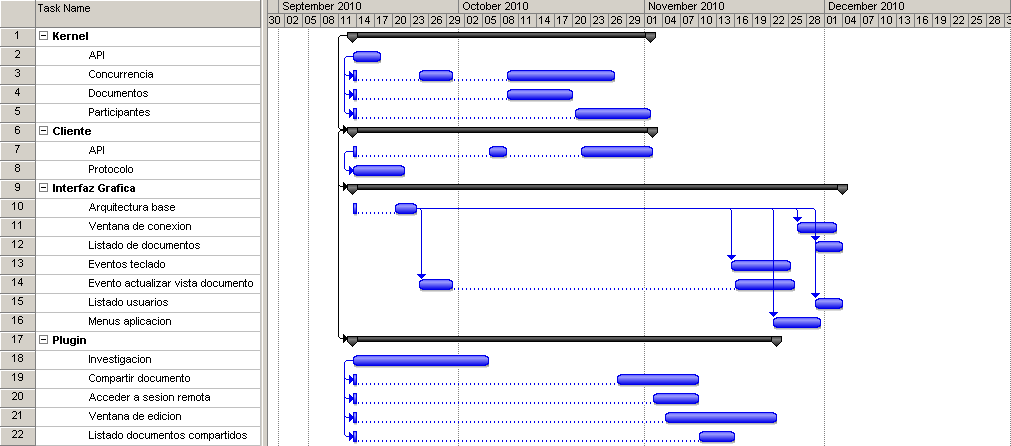
\includegraphics[width=14cm]{gantt.png}
			\caption{\label{gantt} Gantt }
		\end{center}
	\end{figure}

	El gráfico no incluye el buffer agregado al final. Se planificaron 3HH/dia/recurso productivas y el diagrama fue armado siguiendo este valor. La jornada de cada día fue realizada con esa cantidad de horas.

	Este diagrama representa una guía para la organización y planificación de las tareas que serán llevadas a cabo para completar el proyecto. La planificación definitiva de las mismas se realizará con mayor precisión al inicio de cada sprint (sprint planning meeting) incluyendo primero aquellas tareas que agreguen mayor valor en cada iteración y generen una versión usable del producto al finalizar cada una de las mismas.

	\section{Metodología de desarrollo}
	
	Para el desarrollo del proyecto se aplicará la metodología Scrum.

	Scrum es una metodología agil de desarrollo de software. Se enfoca principalmente en entregar la mayor cantidad de valor al negocio en el tiempo más corto posible teniendo en cuenta las prioridades del cliente. Permite obtener versiones funcionales y operativas del producto en intervalos cortos de tiempo posibilitando el retorno de la inversión del cliente con cada iteración.
	
	En cada iteración se realizan tareas de diseño, desarrollo y prueba. El equipo de trabajo consta de un conjunto de profesionales auto-organizado que determina cual es la mejor forma de completar las tareas para entregar las funcionalidades mas prioritarias.
	
	Cada 2 a 4 semanas se puede ver un incremento funcional en el producto que esta listo para usar y puede decidirse liberarlo en ese momento o continuar mejorándolo en otra iteración. La longitud del sprint se fija en un período tal que sea posible dejar posibles cambios afuera.

	\subsection{Roles}

	Dentro del equipo de trabajo típico de Scrum, existen los siguientes roles:
	
	\begin{itemize}
	\item \textit{Product Owner}: decide cuales son las características del producto. Es el responsable de definir cuales serán las prioridades de la iteración tratando de maximizar el retorno de la inversión. Aprueba o rechaza el trabajo realizado.

	\item \textit{Equipo Scrum}: es el equipo auto-organizado multidisciplinario de personas que se encargan de la ejecución de las tareas que se planifican para cada sprint.

	\item \textit{Scrum Master}: es el responsable de la adminsitracion del proyecto. Se asegura que se apliquen los principios de Scrum durante el desarrollo de mismo. Se asegura que el equipo de trabajo sea totalmente funcional y productivo. Aisla al equipo de interferencias externas y elimina los impedimentos para que puedan completar sus tareas.
	
	\end{itemize}

	\subsection{Reuniones}
	Durante el desarrollo del proyecto se realizant tres tipos de reuniones:

	\begin{itemize}
	\item \textit{Sprint planning}: se realiza al inicio de cada sprint. Participan el product owner, scrum master y el equipo de trabajo. Se realiza la priorización y seleccion de las tareas y funcionalides que serán desarrolladas durante el sprint a iniciar. Al final de esta reunión se obtiene el objetivo y la planificación del sprint.

	\item \textit{Daily scrum meeting}: la realizan el equipo de trabajo junto con el scrum master. Es una reunión corta y lo mas frecuente posible (idealmente diaria).  Tiene como objetivo poner al tanto al equipo de trabajo de las tareas que esta realizando cada integrante y de los problemas que surgieron.

	\item \textit{Sprint Review}: Se realiza al final de cada sprint. El equipo muestra el resultado del trabajo desarrollado. Toma generalmente la forma de una demostración de las funcionalidades logradas. Participan el cliente, product owner, scrum manager y el equipo scrum.

	\item \textit{Sprint Retrospective}: participan exclusivamente los miembros del equipo Scrum. Se exponen lecciones aprendidas a lo largo del sprint que termino y se toman decisiones sobre aspectos a conservar o cambiar de la forma de trabajo.
	\end{itemize}


	\subsection{Documentación}
	Al finalizar cada sprint se dispondrá de la siguiente documentación.

	\begin{itemize}
		\item Informe de avance.
		\item Funcionalidades desarrolladas.
		\item Indicador de cobertura de la prueba. Detalle que porcentaje y que partes del código fuente fueron alcanzados por los test unitarios.
		\item Estado de los tests funcionales.
		\item Resultado de los tests que se ejecutaron.
		\item Burndown chart (ver \cite{burndown}).
	\end{itemize}

	\section{Criterios de calidad}
	
Se realizarán dos tipos de pruebas sobre el producto una vez iniciado el desarrollo. Como primer tipo se realizarán pruebas unitarias sobre el código fuente desarrollado. El objetivo es encontrar problemas en la lógica de la aplicación y a su vez documentar indirectamente el uso de la API.

	El porcentaje del código fuente que se pretende cubrir con las pruebas unitarias es del 60\%. El foco de las pruebas se concentrará en los módulos núcleo y cliente del producto.

	El segundo tipo de prueba a realizar son las pruebas funcionales. Estas tienen como característica que son dificilmente automatizables y deben ser realizadas por el usuario que utilizara la aplicación. Las pruebas se correrán al finalizar cada uno de los sprints definidos en la planificación de modo que funcionalidades ya desarrolladas no sean afectadas.

La definición de las pruebas a ejecutar se realizará al inicio de cada sprint.	
	
	\section{Tecnologías}
	
	\begin{itemize}
	
	\item Scala: para el desarrollo de los módulos cliente, núcleo e interfaz gráfica se utilizará el lenguaje de programación Scala. El mismo está diseñado teniendo en mente concurrencia, expresividad y escalabilidad. El resultado de la compilación produce código objeto que corre sobre la máquina virtual de java, aprovechando la estabilidad y madurez de la misma. Provee un modelo de comunicación por mensajes basado en actores que simplifica y abstrae de los problemas clásicos que surgen de la naturaleza concurrente del dominio.
Se eligió este lenguaje ya que ofrece una visión alternativa a los problemas clásicos de la concurrencia y será de soporte principalmente para el núcleo de la aplicación.

	\item Java: el lenguaje Scala permite utilizar código Java y viceversa. El plugin que se desarrollará para el IDE Eclipse será desarrollado con el lenguaje Java, ya que Eclipse se encuentra desarrollado en esa plataforma.

	\item Spring: framework para la inyección de dependencias.

	\item Maven: herramienta para la la gestión y automatización de los procesos del ciclo de vida del proyecto en términos de compilación, dependencias, tests, integración, etc.

	\item Framework de unit testing: Scala Test y TestNG.

	\item Versionado GIT: sistema de versionado de código distribuído.

	\item Eclipse IDE: es el estandar de facto entre los entornos de desarrollo integrado para Java.

	\item GitHub: el código fuente será alojado en este sitio. El sitio provee gráficos y estadísticas útiles sobre el desarrollo del código fuente.	

	\end{itemize}

	
	\section{Infraestructura necesaria}

Para la utilización del producto se requerirá la siguiente infraestructura de base.
Se distinguirán 2 tipos de configuraciones según la modalidad en la cual se haga uso del producto.
En primer lugar, para el caso del modo peer-to-peer solo será necesario disponer de las terminales o puestos de trabajo que deseen participar de una sesión de edición junto con una conexión de red que soporte el conjunto de protocolos TCP/IP entre las mismas. No es necesario un servidor central o dedicado.

Los requerimientos para correr el producto son equivalentes a aquellos necesario para correr un entorno de desarrollo convencional.

En la figura \ref{peer} se observa un posible escenario reflejando la arquitectura peer-to-peer:


	\begin{figure}[!ht]
		\begin{center}
			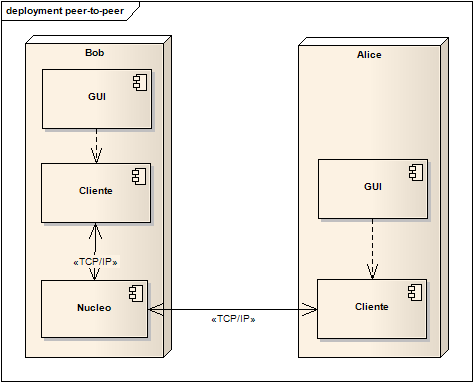
\includegraphics[width=7cm]{peer-to-peer.png}
			\caption{\label{peer} Peer-to-Peer }
		\end{center}
	\end{figure}



En el segundo caso, se dispone de una arquitectura cliente-servidor en la cual participa un servidor dedicado corriendo el Núcleo de la aplicación y los distintos clientes que se conectan con el mismo. La conexión se establece entre el componente cliente y el componente núcleo abstrayendo a la aplicación GUI de la complejidad subyacente.

Se puede ver en la siguiente figura:

	\begin{figure}[!ht]
		\begin{center}
			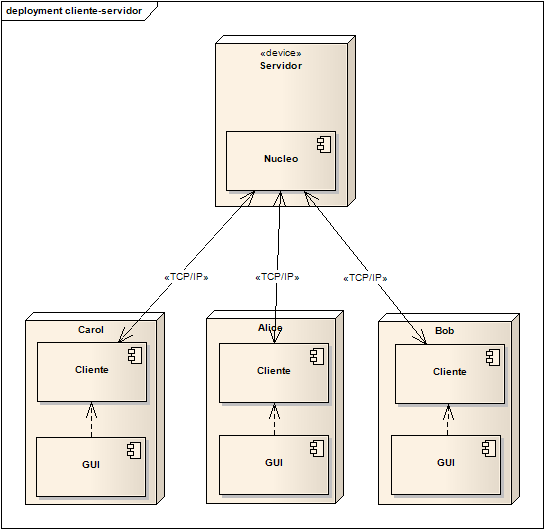
\includegraphics[width=7cm]{cliente-servidor.png}
			\caption{\label{server-client} Cliente-Servidor }
		\end{center}
	\end{figure}

Esta alternativa permite concentrar todos los documentos que editan los usuarios en un solo punto.

En ambos casos no se necesita conectividad internet.	
	
	\section{Riesgos}

A continuación se hará una lista de riesgos que fueron relevados al inicio del desarrollo del proyecto.

\begin{center}
    \begin{tabular}{ | l | p{5cm} | l | l | l | p{5cm} |}
    \hline
    ID & Riego & P & I & E & Plan de mitigación \\ \hline

	1 & Demoras en el desarrollo de las funcionalidades por la poca experiencia en el desarrollo con Scala.
	& 2 & 3 & 6 &
	Retrasar el desarrollo para incorporar conocimientos sobre las herramientas.
	Cambiar la herramienta por otra en la que se tenga mayor epxepriencia. \\ \hline

	2 & Demoras en el desarrollo de la integración con Eclipse debido al desconocimiento de la arquitectura del mismo.
	& 2 & 2 & 4 &
	Integrar el producto con otro IDE. Incorporar conocimiento acerca de la arquitectura del Eclipse y su integración de plugins. \\ \hline

	3 & Demoras en el proyecto por la no aprobación de la propuesta de trabajo profesional.
	& 1 & 3 & 3 &
	Iniciar la construcción a partir de un subconjunto de requerimientos consensuados. Acordar qué falta definir. Evaluar la posibilidad de incluirlo dentro del proyecto o si es necesaria una ampliación. \\ \hline

	4 & Demoras en la definición de la arquitectura produce retrabajo.
	& 2 & 3 & 6 &
	Realizar una definición temprana de la arquitectura y documentarla. \\ \hline
    \end{tabular}
\end{center}

Los valores usados en las tablas corresponden a las siguientes definiciones: \\

Probabilidad (P): valor numérico entre 1 y 3.

Impacto (I): valor numérico entre 1 y 3.

Exposición (E): P * I.

	\section{Requerimientos funcionales}
	
	Se separaran los requerimientos funcionales segun al modulo al que correspondan.

	\subsection{Núcleo}
	\begin{enumerate}
	\item Resolucion de conflictos: implementación del algoritmo de resolución de conflictos. Se utilizará el algoritmo de Júpiter \cite{jupiter} para resolver el escenario concurrente presente en el producto.
	\item Documentos: implementación de las entidades que mantienen el estado del documento en memoria, mientras los participantes aplican operaciones sobre ellos para agregar o borrar contenido. El núcleo ofrecerá servicios para crear documentos vacíos o para asignar un contenido inicial a documento. El origen de este documento dependerá de la aplicación cliente.
	\item Participantes: los participantes son los usuarios conectados y los cuales pueden observar los documentos que se existen. No existirá restricción en cuanto a que usuarios pueden editar cuales documentos, sino que cualquier usuario podrá suscribirse a un documento para editarlo o ver su contenido.
	
	\end{enumerate}


	\subsection{Cliente}

	\begin{enumerate}
\item Implementacion API Cliente: diseñar e implementar la API que se le ofrecerá a las aplicaciones cliente para que hagan uso de los servicios ofrecidos por el producto.
A su vez, es necesario implementar el protocolo de comunicación con el núcleo para el envío y recepción de mensajes en ámbos sentidos.

\item Notificacion de eventos: ofrecer una abstracción a la aplicación que use esta API para manejar los eventos hacia y desde el núcleo. Los eventos que se enviarán son los correspondientes al ingreso de texto en la aplicación cliente y los eventos que se reciben son los que se originan en los otros participantes de la sesión de edición.

\item A su vez se deberan atender otro tipo de eventos tales como: mensajes de chat, mensajes de ingreso o egreso de algún participante a la sesión de edición, etc.
	\end{enumerate}

	\subsection{GUI} 
	Se requiere una aplicación gráfica que permita las siguientes funcionalidades:
	\begin{enumerate}
	\item Crear sesiones de edicion.
	\item Conectar a una sesion de edicion.
	\item Ver documentos disponibles para edicion una vez que se ha conectado a un servidor.
	\item Crear documento de texto vacio.
	\item Compartir documento local para edicion colaborativa con otros participantes.
	\item Guardar el documento en edición.
	\item Editar un documento de texto.
	\item Listar usuarios que se encuentran en la sesión de edición.
	\item Desconectar sesion de edicion.
	\end{enumerate}


\subsection{Plugin}
Se requiere un modulo plug-in para la incorporación a un entorno integrado de desarrollo de las siguientes fuincionalidades:
	\begin{enumerate}
	\item Compartir documento actual para edición colaborativa.
	\item Conectarse a sesión de edicion.
	\item Desconectarse de sesión de edición.
	\item Editar documentos.
	\end{enumerate}
	\section{Requerimientos no funcionales}


\subsection{Integrabilidad} Se garantizará implementando dos interfaces de usuario distintas (GUI y Plugin) que hagan uso del mismo código base, solamente desarrollando las funcionalidades necesarias o distintas para cada caso.
Por otra parte, se definirá y documentará una API de modo que pueda ser incorporado a otros productos por terceras partes.

\subsection{Seguridad} El producto para esta primer versión utilizará un protocolo de texto plano, en el cual se podrá ver toda la información transmitida entre los clientes. Si se pretende transmitir información sensible se deberá añadir una capa que permita el cifrado de la comunicación. Se buscará que esta capa adicional de seguridad sea fácilmente incorporable al producto.

\subsection{Confiabilidad} Los usuarios deberán poseer una versión consistente del documento que se encuentran editando. Al finalizar la sesión de edición todos los participanates deben poseer la misma version de documento. Para garantizar este requerimiento se realizarán pruebas unitarias exhaustivas sobre el núcleo de la aplicación, ya que este es el encargado de aplicar el mecanismo de resolución de conflictos.

\subsection{Portabilidad} Se buscará hacer que el desarrollo sea compatible con las principales plataformas, para esto se realizará sobre la máquina virtual de java aprovechando que cuenta con implementaciones para distintas arquitecturas.	
	
	\section{Entregables}

	\begin{itemize}
	\item Manual de usuario: contendrá la descripción y la forma de utilización de las funcionalidades de la GUI y el Plugin. Para los otros módulos se entregará la documentación técnica referente a la API.
	\item Manual técnico: se desarrollará el manual técnico para los módulos Núcleo y Cliente. Se incluirá documentación sobre la arquitectura, despliegue, los principales módulos, principales puntos de extensión.
	\item Plan de proyecto: el presente documento y la información de avance para cada sprint.
	\item Software: el producto listo para despliegue en CD.
	\end{itemize}

	\section{Glosario}



\begin{itemize}

\item \textbf{API}: una interfaz de programación de aplicaciones o API (del inglés application programming interface) es el conjunto de funciones y procedimientos (o métodos, en laprogramación orientada a objetos que ofrece cierta biblioteca para ser utilizado por otro software como una capa de abstracción. Usados generalmente en las bibliotecas.

\item \textbf{IDE}: entorno de programación que ha sido empaquetado como un programa de aplicación, es decir, consiste en un editor de código, un compilador, un depurador y un constructor de interfaz gráfica (GUI). Los IDEs pueden ser aplicaciones por sí solas o pueden ser parte de aplicaciones existentes.

\item \textbf{Plugin}: Un complemento es una aplicación que se relaciona con otra para aportarle una función nueva y generalmente muy especifica. Esta aplicación adicional es ejecutada por la aplicación principal e interactúan por medio de la API.

\item \textbf{WBS}: estructura de descomposición del trabajo o EDT, también conocido por su nombre en inglés Work Breakdown Structure o WBS, es una estructura exhaustiva, jerárquica y descendente formada por los entregables a realizar en un proyecto. La EDT es una herramienta muy común y crítica en la gestión de proyectos.

\item \textbf{Diagrama de Gantt}: es una popular herramienta gráfica cuyo objetivo es mostrar el tiempo de dedicación previsto para diferentes tareas o actividades a lo largo de un tiempo total determinado. A pesar de que, en principio, el diagrama de Gantt no indica las relaciones existentes entre actividades, la posición de cada tarea a lo largo del tiempo hace que se puedan identificar dichas relaciones e interdependencias.

\item \textbf{Burndown Chart}: es una representación gráfica del trabajo por hacer en un proyecto en el tiempo. Usualmente el trabajo remanente (o backlog) se muestra en el eje vertical y el tiempo en el eje horizonal. Es decir, el diagrama representa una serie temporal  del trabajo pendiente. Este diagrama es útil para predecir cuándo se completará todo el trabajo. Usualmente se usa en el desarrollo ágil de software, especialmente con Scrum.

\end{itemize}


\newpage
\begin{thebibliography}{9}
	\bibitem{visiontpprof}
	Ciancio, Gilioli,
	\emph{Visión Trabajo Profesional}.
	Facultad de Ingeniería.
	Universidad de Buenos Aires. 

	\bibitem{jupiter}
	Nichols, Curtis, Dixon and Lamping,
	\emph{High-Latency, Low-Bandwidth Windowing in the Jupiter Collaboration System}.
	Xerox PARC

	\bibitem{ide}
	Entorno de desarrollo integrado. \\
	http://es.wikipedia.org/wiki/Entorno\_de\_desarrollo\_integrado

	\bibitem{wbs}
	WBS - Work breakdown structure. \\
	http://en.wikipedia.org/wiki/Work\_breakdown\_structure

	\bibitem{gantt}
	Diagrama de Gantt. \\
	http://es.wikipedia.org/wiki/Diagrama\_de\_Gantt

	\bibitem{burndown}
	Burndown chart. \\
	http://es.wikipedia.org/wiki/Burn\_down\_chart
	
	%agregar referencia a scrum

\end{thebibliography}

\end{document}